\documentclass{scrartcl}
\usepackage{../brendan}

% fix spacing
\RedeclareSectionCommand[beforeskip=-2.8ex plus -0.8ex minus -0.2ex, afterskip=1.2ex plus 0.2ex]{section}
\RedeclareSectionCommand[beforeskip=-2.6ex plus -0.8ex minus -0.2ex, afterskip=1.0ex plus 0.2ex]{subsection}
\RedeclareSectionCommand[beforeskip=-2.6ex plus -0.8ex minus -0.2ex, afterskip=1.0ex plus 0.2ex]{subsubsection}
\tcbset{btbox/.append style={before skip=0.5\baselineskip, after skip=0.5\baselineskip}}

% unbold subtitle
\setkomafont{subtitle}{\normalfont\large\color{HeadSlate!85}}

% units
\newcommand{\unit}[1]{\,\text{\small #1}}

% this genuinely took forever to get right
\newcommand{\answerbox}[1]{\tcbox[on line, colback=ThmBlue!9, colframe=ThmBlue!65,  boxrule=0.6pt, arc=2pt, left=4pt, right=4pt, top=2pt, bottom=2pt]{$\displaystyle #1$}}
% now imagine trying to use tikz
% oh wait thats next deliverable
% kill me now

\newcommand{\journalname}{Journal of N$\Psi$ Bridge Design}
\subject{\journalname}
\setkomafont{subject}{\normalfont\large\scshape\color{HeadSlate!85}}
\title{Call for Abstracts}
\renewcommand{\thetitle}{\journalname: Call for Abstracts}
\hypersetup{pdftitle={Journal of N$\Psi$ Bridge Design: Call for Abstracts}}

\subtitle{Team 809 \quad$\star$\quad TA: Mohi}
\author{Daniel Kessler, Cary Li, Zekai Liu, Brendan Tang, Leon Zhang}
\date{\today}

\begin{document}
\ihead{\textsc{Team 809}}
\maketitle
\begin{foreword}
    The style for this document is a heavily modified version of \href{https://github.com/vEnhance}{Evan Chen}'s \texttt{evan.sty}. Attribution is included in the \texttt{.sty} file for this document, as required. 
\end{foreword}
\tableofcontents

\newpage

\section{Shear Force and Bending Moment Diagrams}
\begin{note}
    We make the following simplifications:
    \begin{enumerate}
        \item The self-weight of the bridge is neglected
        \item Applied loads are treated as point loads
    \end{enumerate}
\end{note}

\bigskip
Here is the bridge:

% top images
\noindent
\begin{minipage}[t]{0.48\linewidth}
    \vspace{0pt}
    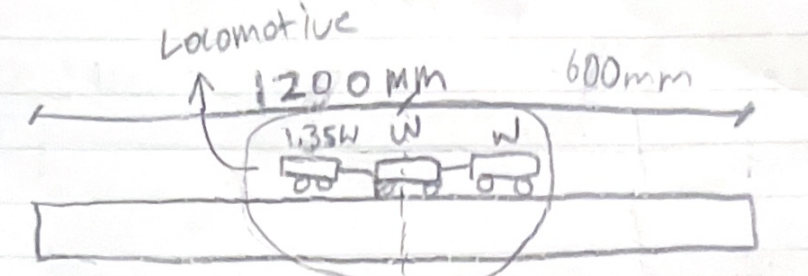
\includegraphics[width=\linewidth]{../images/img1.png}
\end{minipage}\hfill
\begin{minipage}[t]{0.48\linewidth}
    \vspace{0pt}
    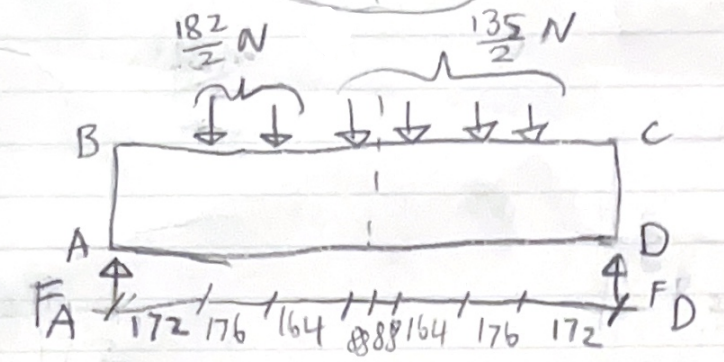
\includegraphics[width=\linewidth]{../images/img2.png}
\end{minipage}

\bigskip

% equations
\noindent
\begin{minipage}[t]{0.48\linewidth}
    \vspace{-4.5em}
    \[
        \begin{aligned}[t]
            \sum M_{A}&=0 \\
            0&=1200F_{D}-172(91)-348(91)\\&-512(67.5)-688(67.5)\\&-852(67.5)-1028(67.5) \\
            F_{D}&=\answerbox{213\unit{N}}\,\text{,}
        \end{aligned}
    \]
\end{minipage}\hfill
\begin{minipage}[t]{0.48\linewidth}
    \[
        \begin{aligned}[t]
            \sum F_{Y}&=0 \\
            F_{A}&=182+2(135)-F_{D} \\
            F_{A}&=\answerbox{239\unit{N}}\,\text{.}
        \end{aligned}
    \]
\end{minipage}

\bigskip

Thus, we get the following diagrams:

% SFD & BMD
\noindent
\begin{minipage}[t]{0.48\linewidth}
    \vspace{0pt}
    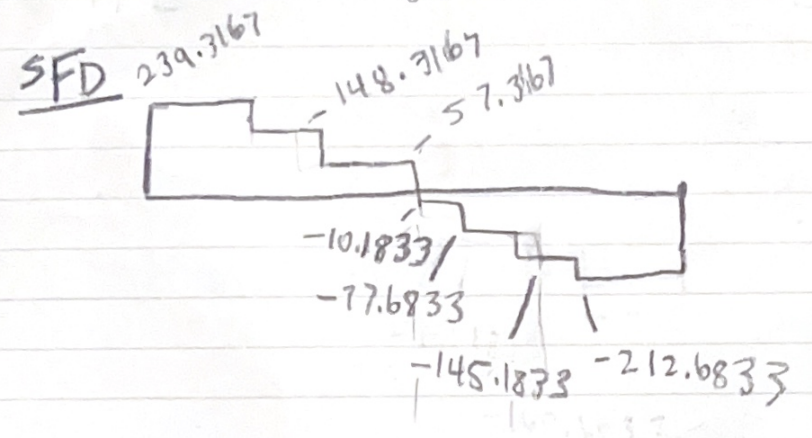
\includegraphics[width=\linewidth]{../images/sfd_REAL.png}
\end{minipage}\hfill
\begin{minipage}[t]{0.48\linewidth}
    \vspace{0pt}
    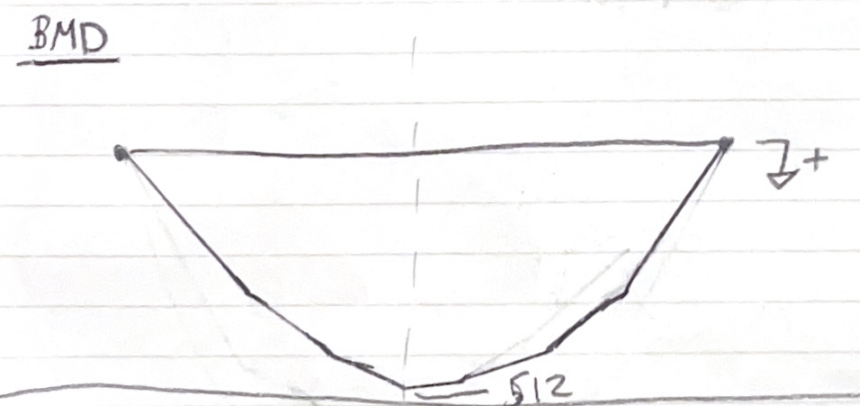
\includegraphics[width=\linewidth]{../images/sfd.png}
\end{minipage}

\bigskip

\begin{remark}
    Due to \href{https://tikz.dev}{TikZ} being extraordinarily unintuitive to use, all diagrams in this deliverable will be drawn by hand. 
\end{remark}

\newpage

\section{Centroidal Axis and Moment of Inertia}

Here is a cross-sectional view. All rectangular pieces are uniform. All lengths are in$\unit{mm}$ and all areas are in$\unit{mm\textsuperscript{2}}$.

\bigskip
\noindent
\begin{minipage}[t]{0.48\linewidth}
    \vspace{0pt} % fixes equations :)
    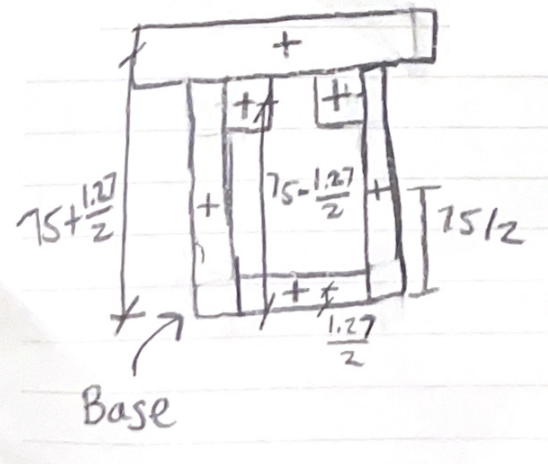
\includegraphics[width=\linewidth]{../images/crossy.png}
\end{minipage}\hfill
\begin{minipage}[t]{0.48\linewidth}
    \vspace{-\abovedisplayskip}\vspace{0.5em}
    \[
        \begin{aligned}[t]
            A_{\text{glue tab}} &= 5(1.27) = \answerbox{6.35\unit{mm\textsuperscript{2}}} \\
            A_{\text{side}} &= 75(1.27) = \answerbox{95.3\unit{mm\textsuperscript{2}}} \\
            A_{\text{top}} &= 100(1.27) = \answerbox{127.0\unit{mm\textsuperscript{2}}} \\
            A_{\text{bottom}} &= \bigl(80-2(1.27)\bigr)(1.27) \\
              &= \answerbox{98.4\unit{mm\textsuperscript{2}}}
        \end{aligned}
    \]
\end{minipage}

Thus,
\[
\begin{aligned}
    \bar{y} &= \frac{\sum A_i \, y_{i\,b}}{\text{Total Area}} \\[0.6em]
    &= \frac{2(6.35)(74.365) + 2(95.25)(37.5) + 127(75.635) + 98.3742(0.635)}{2(6.35) + 2(95.25) + 127 + 98.3742} \\[0.6em]
    &= \frac{17756.2981}{428.5742} \\[0.6em]
    &= 41.43\unit{mm} \\[0.3em]
    \bar{y} &= \answerbox{41.4\unit{mm}}
\end{aligned}
\]
and
\[
\begin{aligned}
    I_{\text{total}} &= 2\left(\frac{5(1.27)^3}{12}\right) + 2\left(\frac{1.27(75)^3}{12}\right) + \frac{77.46(1.27)^3}{12} \\
    &\quad + \frac{100(1.27)^3}{12} + 2\bigl(6.35(32.935)^2\bigr) + 2\bigl(95.25(3.93)^2\bigr) \\
    &\quad + 127(34.205)^2 + 98.3742(40.795)^2 \\[0.3em]
    &= 89328.87416 + 329023.3354 \\
    &= 418352\unit{mm\textsuperscript{4}} \\[0.3em]
    I &= \answerbox{4.18 \times 10^{5}\unit{mm\textsuperscript{4}}}\,\text{.}
\end{aligned}
\]

\section{Factors of Safety}

\noindent
\begin{minipage}[t]{0.23\linewidth}
    \vspace{0pt}
    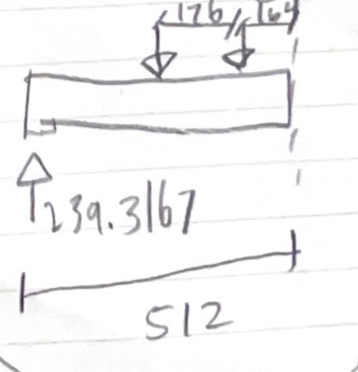
\includegraphics[width=\linewidth]{../images/mini.png}
\end{minipage}\hfill
\begin{minipage}[t]{0.73\linewidth}
    \vspace{0pt}
    From the BMD, $M$ is largest at $x=512\unit{mm}$. Hence, we cut the beam at $x=512\unit{mm}$:
    \begin{align*}
        \sum M_{x=512} &= -512(239.3167) \\
        &\quad + 91(164) + 91(340) \\
        M_{x=512} &= \answerbox{76700\unit{N\,mm}}
    \end{align*}
\end{minipage}

The bottom is in tension:
\begin{align*}
    \sigma &= \frac{M_{\max}\, y}{I} = 7.59236\unit{MPa} \\[0.5em]
    \therefore\text{FoS}_{\text{tens.}} &= \frac{30}{\sigma} = \answerbox{3.95}\,\text{.}
\end{align*}

The top is in compression:
\begin{align*}
    \sigma &= \frac{M_{\max}\,(76.27 - 41.43)}{I} = 6.38469\unit{MPa} \\[0.5em]
    \therefore\text{FoS}_{\text{comp.}} &= \frac{6}{\sigma} = \answerbox{0.940}\,\text{.}\quad\text{(bad)}
\end{align*}

\begin{remark}
    While all boxed numbers are formatted with slide-rule precision, we used their unrounded values whenever they appeared in calculations.
\end{remark}

\end{document}